\chapter{L’impact d’un projet aux acteurs multiples sur l’intégrité des données}

La donnée occupe une place centrale dans le projet, à la fois comme objectif ultime et comme matière première de toute la chaîne de traitement. Il est donc essentiel de saisir sa nature et son rôle à chaque étape du projet. Comprendre la nature des données conduit inévitablement à s'interroger sur leur statut juridique : à qui appartiennent-elles et comment s’inscrivent-elles dans le cadre légal des archives ? Par la suite, nous examinerons le parcours des données, manipulées par diverses équipes à l’aide de plusieurs outils, ce qui met en lumière la dimension interdisciplinaire du projet. Enfin, nous analyserons l'intégration des données dans la base, en soulignant les défis techniques et organisationnels liés à la gestion d’un volume important d’informations.   

    \section{L'aspect juridique : à qui appartient la donnée}

De façon générale, les archives publiques sont communicables de plein droit (article L213-1 du code du patrimoine)\footnote{\href{https://www.legifrance.gouv.fr/codes/article_lc/LEGIARTI000031971829}{Article L213-1 du code du patrimoine}}. Une archive publique est une archive produite par un organisme de l’administration ou chargé d’une mission de service public. C’est bien évidemment le cas pour les listes de recensement, puisqu’elles sont produites jusqu’en 1946 par le Bureau de la statistique, puis par l’INSEE. Cependant ces archives peuvent être communiquées, selon un délai qui est déterminé davantage par la nature de la donnée que par le type de document. Selon l’article 213-2 du code du patrimoine\footnote{\href{https://www.legifrance.gouv.fr/codes/article_lc/LEGIARTI000043887707}{Article L213-2 du code du patrimoine}}, les délais de communicabilité varient : les documents produits par une administration sont communicables après 25 ans, mais ce délai est porté à 50 ans pour les documents portant atteintes à la vie privée.\\
En principe, on devrait donc se demander si les listes de recensement portent atteinte à la vie privée d’un individu. Ces listes contiennent son adresse, sa date de naissance et la composition de son foyer. On pourrait arguer que c’est une photographie à un instant T et que ça peut ne pas lui poser préjudice. Pour éviter ce genre de débat, un arrêté a été pris, par dérogation au code du patrimoine :

\begin{quote}
    \textit{"Peuvent être librement consultées, à des fins de statistique publique ou de recherche scientifique ou historique, les listes nominatives établies par les maires à l'occasion des recensements généraux de la population jusqu'en 1975."\footnote{\href{https://www.legifrance.gouv.fr/jorf/id/JORFTEXT000021467019}{Arrêté du 4 décembre 2009 portant dérogation générale pour la consultation des listes nominatives du recensement général de la population}}. Le projet SocFace s’inscrit clairement dans ce cas de figure, puisque c’est un projet de recherche scientifique.}
\end{quote}

Mais la question est plus complexe que cela. Car le projet SocFace n’est pas qu’un projet qui travaillerait sur les listes de recensement. Les listes de recensement sont généralement utilisées pour des recherches sur l’histoire locale, ou une histoire comparative. Parce que l’entrée principale se fait par année et par commune. Mais elles sont difficiles à manier, et demandent un gros travail d’indexation préalable, nécessairement manuel. Ce type de recherche se base sur l’analyse de la donnée. Le projet SocFace est fondé sur une utilisation de cette donnée : on la récupère pour la faire intégrer la base de données. Selon l’article 2 de l’arrêté autorisant la communicabilité des listes de recensement : \textit{"L’exercice de ce droit ne s’accompagne pas du droit de réutilisation des données, notamment à des fins commerciales"}. La formulation de cette disposition n’est pas très claire. Qu’est-ce que le droit de réutilisation des données ? Quelle différence avec une simple utilisation ? On peut penser que la réutilisation serait une forme d’altération de la donnée. La différence avec une utilisation classique est le fait de l’utiliser dans un cadre différent. Est-ce qu’une base de données est un cadre différent ? il n’y a pas de modification de la nature de la donnée. Les noms, les communes, les dates restent les mêmes. Le seul changement est un réagencement de la lecture de ces données. Par ailleurs, la loi semble pointer du doigt spécifiquement les utilisations commerciales. Il est en effet possible pour une entreprise privée d’utiliser des données publiques pour développer ses activités. Les listes de recensement peuvent intéresser grandement les entreprises de généalogies, qui est une activité très prisée. Le législateur cherchait peut-être à empêcher ces sites de privatiser les listes du recensement. Or le projet SocFace ne compte pas faire payer les utilisateurs de la base de données. Ce projet est un projet de recherche et n’est pas un projet à des fins commerciales. Enfin, il faut rappeler que la production de cette base de données n’est pas le seul objectif du projet. Une fois qu’elle sera opérationnelle, le but est de réaliser des appariements, ou linking, afin d’établir les trajectoires géographiques et sociales d’individus ou d’ensemble d’individus. Il y a donc une visée de recherche même avec l’utilisation des données.\\
Au vu des dispositions peu claires, du fait que c’est plutôt une orientation commerciale qui est interdite et que la réutilisation des données est elle-même à des fins de recherche, on peut penser que SocFace est en accord avec les dispositions juridiques sur l’utilisation des données issues des listes de recensement. Concernant la propriété des données, ce sont des données publiques et dès lors appartiennent à la collectivité, qu’elles soient contenues dans leur source primaire ou dans une base de données. En revanche, la base de données appartient à son producteur, qui détient le droit sur la façon dont sont agencées et présentées les données.\\

Si la compréhension du cadre juridique offre une base nécessaire à l’étude de la donnée, c’est le chemin emprunté par les données, depuis leur collecte jusqu’à leur intégration dans la base de données, qui permet de véritablement saisir les défis techniques et organisationnels associés à ce projet interdisciplinaire. Nous allons donc explorer le parcours de ces données, en mettant en lumière les étapes clés de leur transformation, les outils utilisés et les collaborations indispensables pour garantir leur qualité et leur intégrité.

    \section{Le chemin de la donnée}

        \subsection{Nature de la donnée}

Si l’on adopte le point de vue de la donnée, dans une forme de personnification, on voit que la donnée est conservée sur différents supports, et sous différentes formes. Selon la coopérative Datactivist\footnote{\href{https://datactivist.coop/fr/}{\textbf{\textit{Coopérative Datactivist}}}}: 
\begin{quote}  
\textit{"les données sont couramment comprises comme les matériaux bruts produits dans l’abstraction du monde en catégories, mesures et toute autre forme de représentation-nombres, caractères, symboles, images, sons, ondes électromagnétiques, bits qui constituent les fondations sur lesquelles l’information et le savoir sont créés."}
\end{quote}

La donnée ne doit donc pas être entendue comme l’information, mais comme le support de l’information. En l’espèce, pour nos listes de recensements, la donnée est constituée d’une série de caractères formant des mots. Les données sont accompagnées de métadonnées. En l’espèce, la donnée est le nom d’un habitant, d’une commune, une année… La métadonnée est une donnée sur la donnée, en l’espèce la date de création de la donnée, ou son emplacement. 
Les données concernées par le projet SocFace sont de nature structurées et finies : 
\begin{itemize}
    \item \textbf{Structurées}, parce que la source elle-même, la liste de recensement, est organisée. L’organisation n’est pas exactement la même sur cent ans, la disposition n’est pas toujours identique, mais dans l’ensemble, les éléments recueillis par les censeurs sont les mêmes et sont entrés de façon organisée ; 
    \item \textbf{Finie}, car il s’agit d’archives, les données sont limitées à un ensemble spécifique. 
\end{itemize}
Ces caractéristiques pourraient indiquer que ces données sont de bonnes qualités et facile à analyser. Pour autant, on parle ici de millions d’entrées, remplies sur cent ans par des humains. Ces données ne sont donc pas sans erreurs et peuvent connaître des lacunes ou des incohérences. Ces erreurs seront répercutées tout au long du parcours de la donnée.
        
        \subsection{Parcours de la donnée}

Les données initiales proviennent des listes de recensement, de grands registres contenant, pour chaque année et chaque commune, les noms des habitants et des membres de leur foyer, classés par rue, ainsi que leur position dans le foyer, leur profession, leur âge (et plus tard, leur nationalité). Ces informations sont numérisées par les services d’archives et converties en images au format .jpeg ou .png. Une fois que leur participation au projet SocFace est validée, ces images sont transférées sur des serveurs, appelés "buckets", utilisant la technologie \gls{IIIF}. Celle-ci permet un accès standardisé et collaboratif aux images numériques, facilitant ainsi le travail conjoint de plusieurs institutions sur les mêmes images. Cependant, tous les services d’archives n’utilisent pas \gls{IIIF}, ce qui peut entraîner des efforts supplémentaires pour SocFace.\\
Ensuite, les images sont importées dans \\Spider{}{}, où elles sont associées à leurs métadonnées. À ce stade, les données sont toujours dans les images numérisées, stockées sur les serveurs de Teklia. C’est dans \Arkindex{} que les données sont véritablement extraites grâce à la technologie d’HTR de Teklia. Bien que les données restent présentes dans les images des livres de recensement, elles sont également extraites sous forme de "mentions" (nom, prénom, âge ou année de naissance, position dans la famille, profession et parfois nationalité) et transférées dans une base de données SQLite. L’outil reconstitue également les foyers (\gls{households}), indiquant les relations familiales et les rôles comme époux, épouse, fils, domestique, etc.\\
Ainsi, les données circulent entre différents supports, gérées par diverses équipes, illustrant la collaboration nécessaire entre les institutions impliquées dans le projet. Une fois que la donnée est extraite, elle intègre une base de données, objectif final du projet.
    
    \section{L'agencement des données au sein de la base de données}

La base de données issue du processus de production est constituée de deux étages : 
\begin{itemize}[label=\textbullet]
    \item Un premier étage, avec, dans une première table, les données brutes, issues des listes de recensement, que l’on appelle « mention des individus », c’est-à-dire, le nom, la profession, l’âge etc…  et une deuxième table avec les métadonnées de chaque registre : l’année, la ville, le lieu de conservation, cote et lien vers le fichier numérisé. 
    \item Un second étage, utilisé dans le cadre des travaux de recherche sur l’appariement (\textit{linking}). 
\end{itemize}
 
Nous nous concentrerons ici sur le premier étage, le second étage n’étant pas encore construit en totalité.\\
Cette base de données est hébergée sur les serveurs de l’INED et l’ensemble des données est estimée autour de 3 To, comme on l'a vu au Chapitre 2. 
\clearpage

\begin{figure}[H]
        \centering
        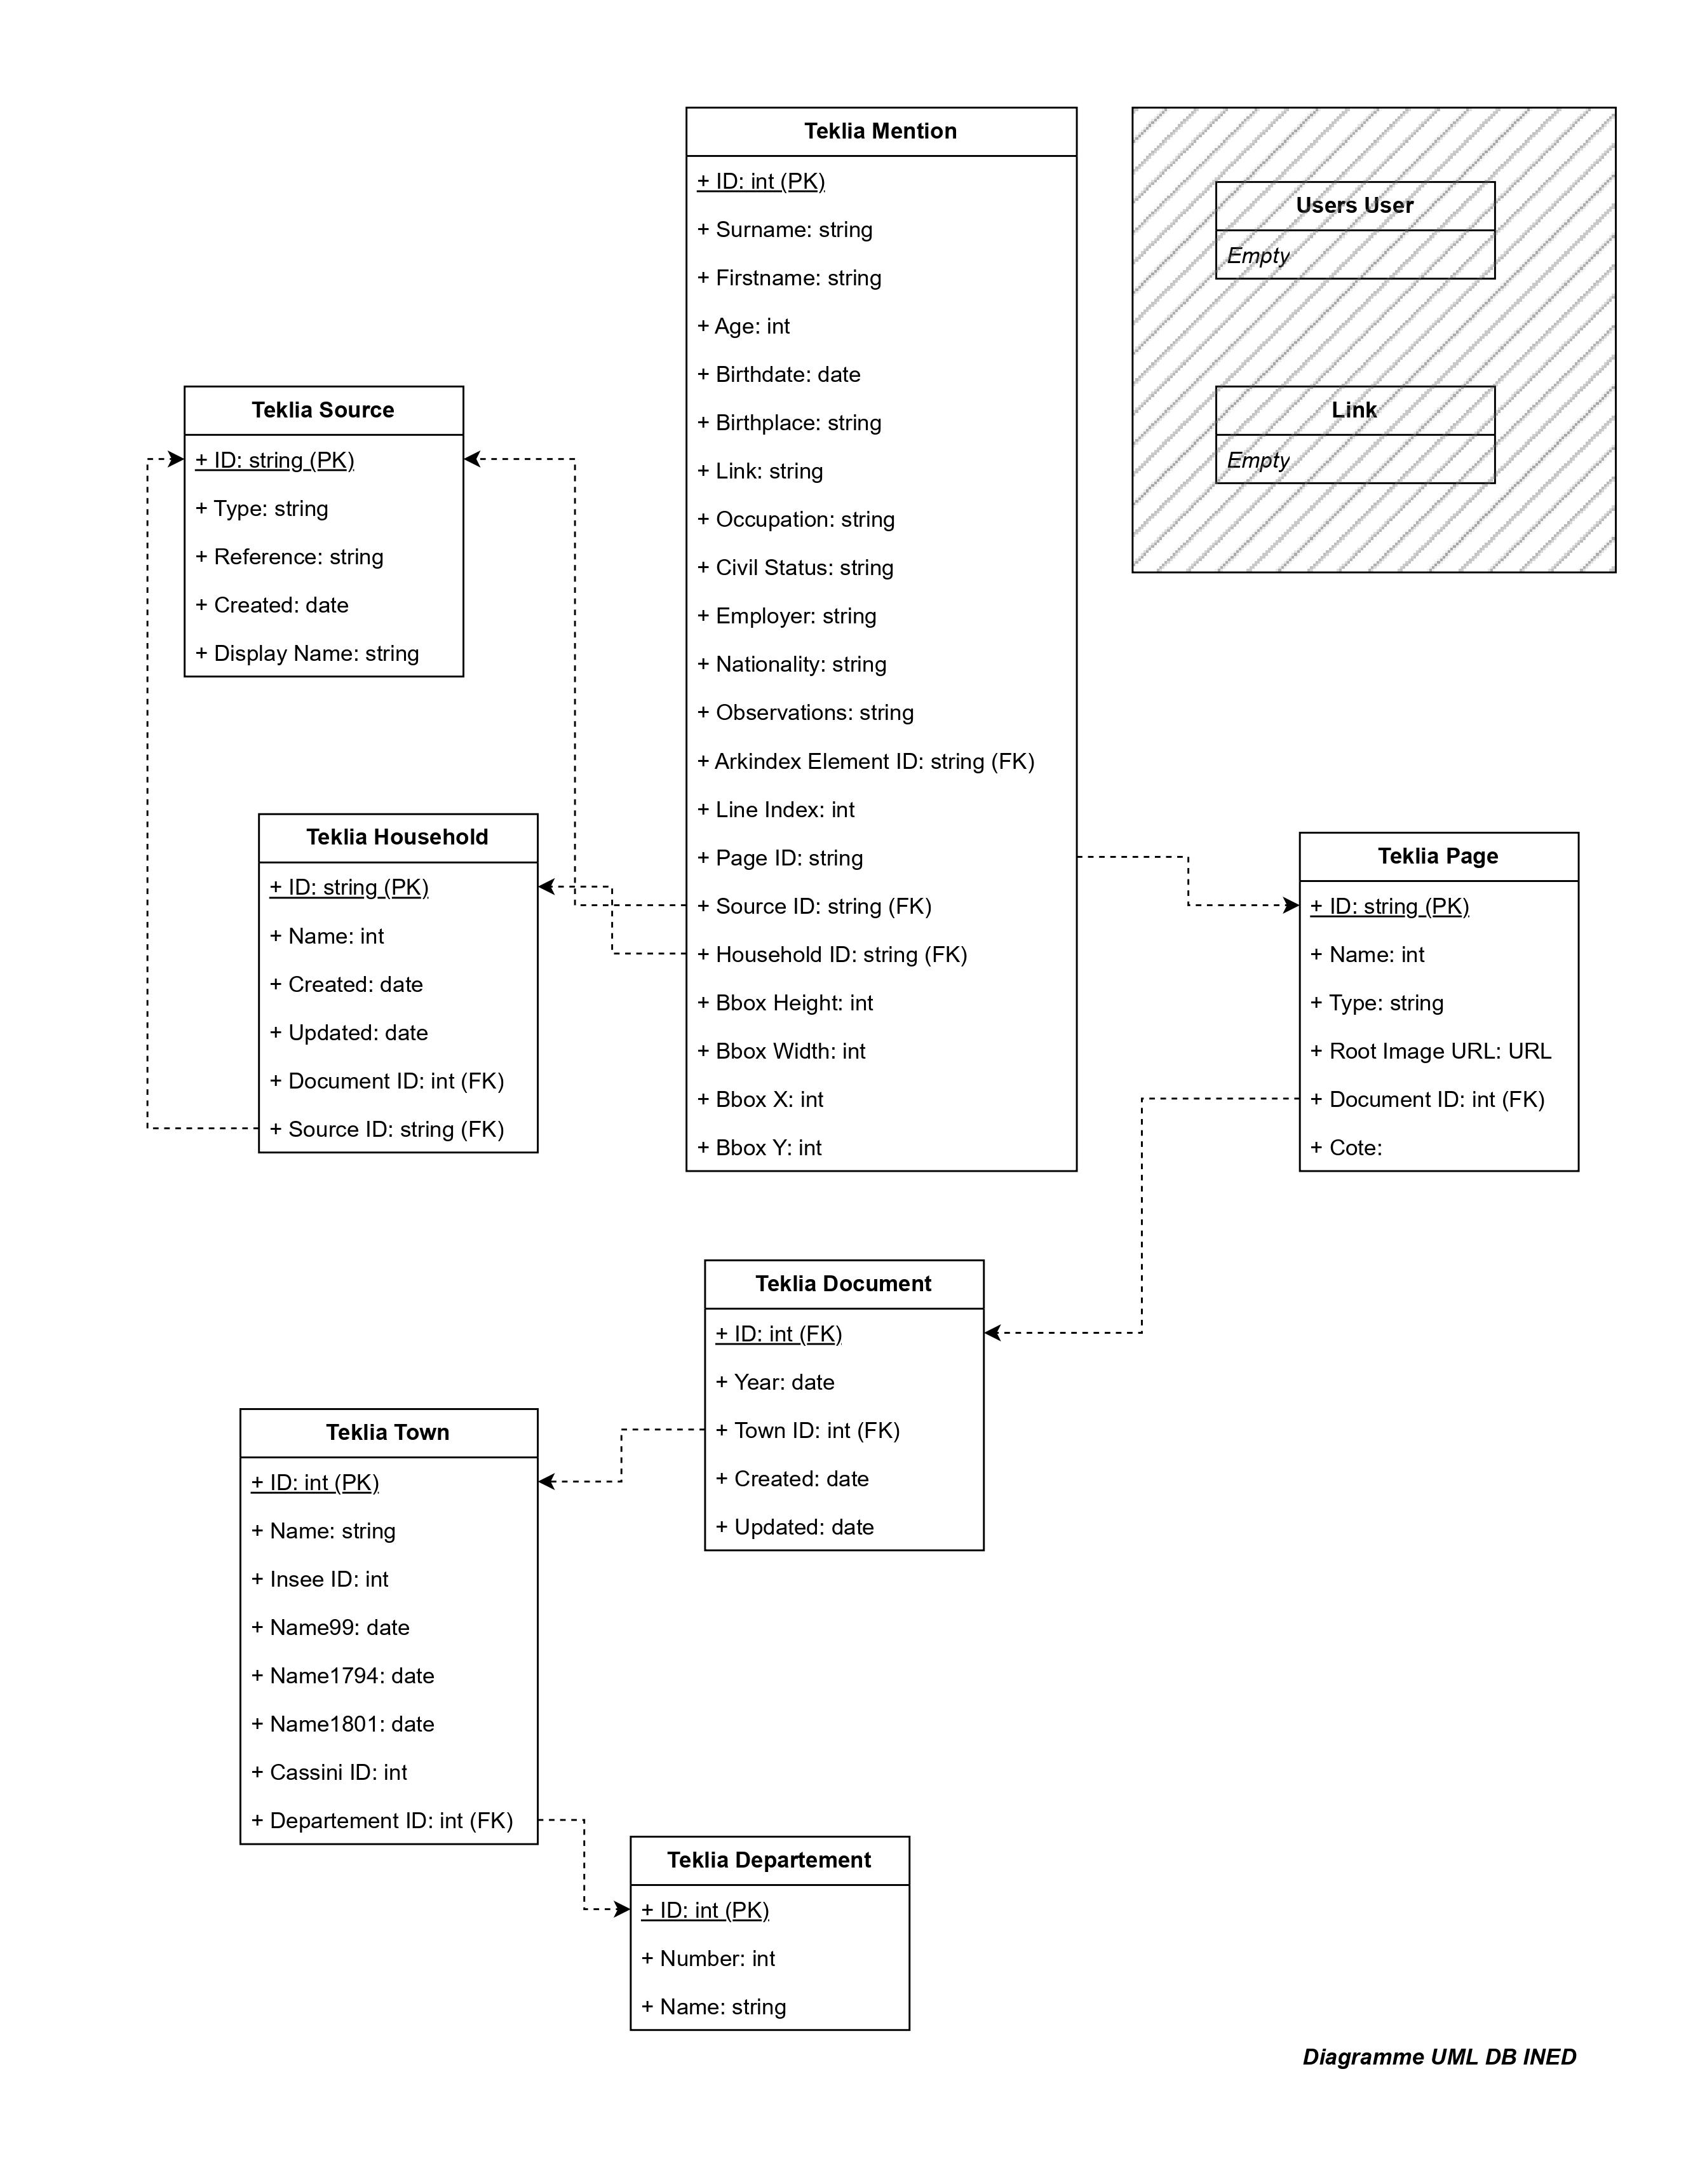
\includegraphics[width=1.0\linewidth]{Figures/Partie 2/Fig.2.1 - Modèle de données - DB INED.jpg}
        \caption[Modèle de données pour la Base de Données]{Modèle de données pour la Base de Données}
        \label{fig:Fig2.1}
    \end{figure}
\clearpage

Plusieurs problèmes vont se poser aux équipes : 
\begin{itemize}[label=\textbullet]
    \item Teklia doit avoir accès à la base de données hébergées sur l’INED pour récupérer les données
    \item Teklia doit pouvoir reverser les métadonnées (collectées par l’outil \\Spider{}{}) dans la base de données de l’INED
    \item FranceArchives (site internet des Archives Nationales) hébergera la base nationale et doit avoir un format pivot interopérable pour reverser les données aux archives départementales et municipales. Pour cela, le SIAF fait appel à un prestataire externe, Logilab.
\end{itemize}

Quelles solutions pour ces problèmes ? 
\begin{enumerate}[label=\alph*)]
    \item \textbf{Concernant le problème de compatibilité entre la base de données de l’INED et celle de Teklia :} 
Pendant un certain temps, les équipes ont réfléchi à la gestion de deux bases de données distinctes : une base de données "\textbf{primaire}" (ou \textit{Master}) et une base de données "\textbf{répliquée}" (ou \textit{slave}). Étant donné que le processus de production est géré par \Arkindex{}, un outil de Teklia, on aurait pu créer la base de données initiale chez Teklia puis la répliquer sur l'INED pour y effectuer les modifications. Ce n'est pas la solution choisie, même si elle aurait tout aussi simple. Mais Teklia verse les données, tandis que l'Ined les travaille et les modifie, il était donc plus logique de procéder ainsi.  
Il y a aussi la solution multimaster, c’est-à-dire dans laquelle les deux bases auraient été considérées comme "\textbf{primary}" et où les écritures peuvent être faites sur les deux avec une synchronisation. Mais cette solution a également été écartée car elle nécessite un logiciel propriétaire et n’est pas très stable, d’autant plus qu’on parle de bases de données d’un poids considérable. 
Il a donc été décidé que la base de données "\textbf{primary}" serait hébergée par l’INED et la "\textbf{replica}" chez Teklia. Un dernier obstacle existait : trouver un système de gestion de base de données compatible sur les deux serveurs. Le choix s’est porté sur PostgresSQL, un modèle répandu et utile pour les bases de données relationnelles. Par ailleurs, les techniciens informatiques de l’INED ont accepté d’ouvrir leurs serveurs à Teklia pour permettre à leurs équipes de travailler dessus et de pouvoir connecter les deux bases pour reverser des données. 
    \item \textbf{Concernant France Archives :}
Dans un premier temps, le SIAF a décidé de travailler à partir d’un "\textbf{dump}". Un "\textbf{dump}" est une sauvegarde d’une base de données (contenu et structure) à un moment donné. La différence avec la réplication c’est que la base n’est pas connectée à la base "\textbf{primaire}", il n’y a donc pas de synchronisation régulière. Mais cela permet au SIAF de commencer à travailler sur la structure de la base, même si les données en elles-mêmes sont amenées à évoluer à mesure que le projet avancera. Par ailleurs c’est une technique beaucoup plus stable, puisqu’il n’y a pas de mises à jour régulières. A terme, le SIAF utilisera un serveur dédié afin d’héberger une réplication de la base de données, afin de la rendre accessible sur leur site internet. 
Ces problèmes techniques découlent de deux éléments: l’ampleur des données traitées, qui nécessite une typologie particulière de serveur et de système de gestion de base de données, et le nombre d’acteurs impliqués, du fait que le projet est interdisciplinaire. Mais en réalité, ces éléments sont liés : l’ampleur des données nécessite une collaboration entre des acteurs aux expertises diverses. Cette collaboration nécessite un travail important sur l’articulation des moyens techniques. Et cette articulation est rendue plus difficile par l’ampleur des données. Un projet monodisciplinaire n’aurait pas connu ces difficultés, car il n'y aurait pas eu d’efforts à faire pour trouver un moyen de partager la base de données à tous les acteurs (dans le cas où il n’y aurait pas de collaboration entre différentes institutions). Ici c’est la collaboration entre plusieurs types de personnes qui pose problème : si le projet n’avait été porté que par l’INED, la base de données serait restée sur leur serveur, et ils auraient pu la gérer comme ils l’entendent, y ajouter des données ou en retirer. Mais ce serait supposer que l’INED possède la technologie suffisante et l’expertise nécessaire pour construire un tel outil. Ce n’est pas le cas et c’est pourquoi ce projet est en collaboration et interdisciplinaire.\\

En résumé, la gestion des données au sein du projet SocFace met en évidence les défis techniques et organisationnels posés par l'ampleur des informations traitées et la diversité des acteurs impliqués. Le caractère interdisciplinaire du projet, essentiel pour exploiter pleinement les compétences de chaque partenaire, complexifie l'articulation des moyens techniques nécessaires. De même, la collaboration entre institutions, bien que cruciale pour le succès du projet, entraîne des difficultés supplémentaires, notamment en ce qui concerne le partage et la synchronisation des données. Il est donc fondamental de développer des solutions adaptées pour assurer la cohérence et l'efficacité de l'ensemble du processus. C’est pour cela que les porteurs du projet ont cherché utiliser un outil de visualisation des données, pour offrir une synthèse claire et accessible des informations collectées à tous les acteurs du projet. Ce type d'outil permet non seulement de suivre l'évolution du projet, mais aussi de fournir aux partenaires, notamment les services d'archives, une représentation visuelle des données traitées.
\end{enumerate}


